% Created 2017-09-25 Mon 14:44
% Intended LaTeX compiler: pdflatex
\documentclass[presentation]{beamer}
\usepackage[utf8]{inputenc}
\usepackage[T1]{fontenc}
\usepackage{graphicx}
\usepackage{grffile}
\usepackage{longtable}
\usepackage{wrapfig}
\usepackage{rotating}
\usepackage[normalem]{ulem}
\usepackage{amsmath}
\usepackage{textcomp}
\usepackage{amssymb}
\usepackage{capt-of}
\usepackage{hyperref}
\usetheme{default}
\author{rob}
\date{\today}
\title{}
\hypersetup{
 pdfauthor={rob},
 pdftitle={},
 pdfkeywords={},
 pdfsubject={},
 pdfcreator={Emacs 24.5.1 (Org mode 9.0.5)}, 
 pdflang={English}}
\begin{document}

\begin{frame}{Outline}
\tableofcontents
\end{frame}

\% Created 2017-09-25 Mon 09:35
\% Intended \LaTeX{} compiler: pdflatex
\documentclass[presentation,9pt,xcolor=dvipsnames]{beamer}
\usepackage[utf8]{inputenc}
\usepackage[T1]{fontenc}
\usepackage{graphicx}
\usepackage{grffile}
\usepackage{longtable}
\usepackage{wrapfig}
\usepackage{rotating}
\usepackage[normalem]{ulem}
\usepackage{amsmath}
\usepackage{textcomp}
\usepackage{amssymb}
\usepackage{capt-of}
\usepackage{hyperref}
\institute{Post-doc (Georgetown University),PhD (Murdoch University)}
\usepackage{tikz}
\usepackage{color}
\usepackage{xcolor}
\usepackage{amsmath}
\usepackage{cancel}
\usepackage{graphicx}
\usetheme[height=7mm]{Rochester}
\usecolortheme[named=Brown]{structure}
\usetikzlibrary{shapes,arrows}
\usetheme{default}
\author{Rob W Rankin}
\date{\today}
\title{Introduction to Bayesian Inference}
\hypersetup\{
 pdfauthor=\{Rob W Rankin\},
 pdftitle=\{Introduction to Bayesian Inference\},
 pdfkeywords=\{\},
 pdfsubject=\{\},
 pdfcreator=\{Emacs 24.5.1 (Org mode 9.0.5)\}, 
 pdflang=\{English\}\}
\begin{document}

\maketitle
\begin{frame}{Outline}
\tableofcontents
\end{frame}

\begin{frame}[label={sec:org5fe48f3}]{outline}
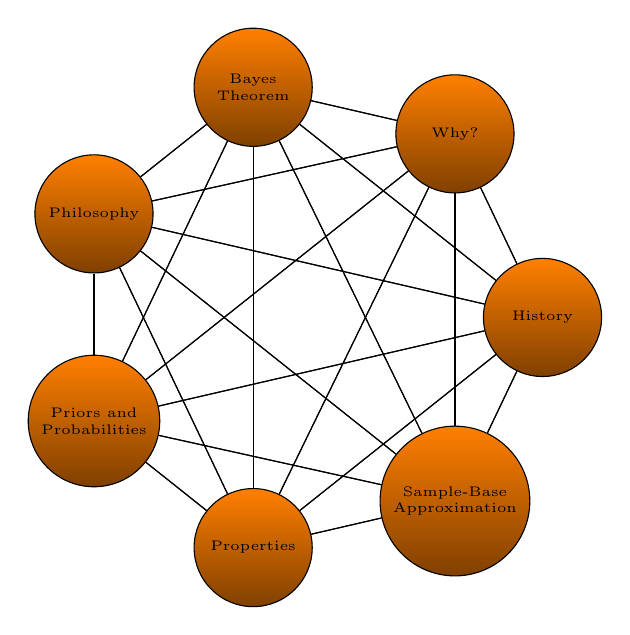
\begin{tikzpicture}
  \foreach \x /\alph/\name in {0/a/History, 51/b/Why?, 103/c/Bayes\\Theorem, 154/d/Philosophy, 206/e/Priors and\\Probabilities, 257/f/Properties, 309/g/Sample-Base\\Approximation}{
    \node[circle, fill=green,minimum width=15mm, draw, font=\tiny, align=center,shading=axis,top color=orange,bottom color =orange!50!black] (\alph) at (\x:3cm) {\name}; }

  \foreach \alpha in {a,b,c,d,e,f,g}%
           {%
             \foreach \alphb in {a,b,c,d,e,f,g}
                      {
                        \draw (\alpha) -- (\alphb);%
                      }
           }
\end{tikzpicture}
\end{frame}
\begin{frame}[label={sec:orgc4bf178}]{Why?}
\begin{block}{why are you interested in Bayesianism?}
\end{block}
\end{frame}
\begin{frame}[label={sec:org8086d8a}]{Why? -- some advantages}
\begin{block}{small sample sizes: exact inference}
\end{block}
\begin{block}{missing data: easy to impute}
\end{block}
\begin{block}{integrate other information}
\end{block}
\begin{block}{derived quantities}
\end{block}
\begin{block}{complex, hierarchical process models}
\begin{block}{multiple sources of variation (space,time)}
\end{block}
\begin{block}{``honest" epistemology}
\end{block}
\end{block}
\end{frame}
\begin{frame}[label={sec:orga96de5b}]{Why? -- some advantages}
\begin{itemize}
\item conditional on the observed data
\item probabilistic statements
\item evidential
\item coherence
\item good frequentist properties
\end{itemize}
-- shrinkage, decision-theory
\begin{itemize}
\item decision making
\end{itemize}
\end{frame}
\begin{frame}[label={sec:orge05d137}]{Why? -- disadvantages}
\begin{itemize}
\item what is probability?
\item language dependence
\item objective basis for science?
\item misalignment between human pschology and probability theory
\end{itemize}
\end{frame}
\begin{frame}[label={sec:orgfbf897c}]{History}
\begin{block}{Neo Bayesian Revival (>1992)}
Gelfand and Smith 1992 - Sampled based approximations of Bayesian posteriors \footnote{MCMC is older, e.g. Metrpolis et al. }
\end{block}
\begin{columns}
\begin{column}{0.6\columnwidth}
\begin{block}{Revival (\textasciitilde{}1920s - )}
\begin{itemize}
\item Subjective Bayesian, Decision Theory
\end{itemize}
Ramsey, De Finetti, Savage, (Wald)
\begin{itemize}
\item Hypothesis Testing, Logical/Objective Bayesism
\end{itemize}
Jeffreys, Jaynes 
\begin{itemize}
\item Hierarchical Bayesian
\end{itemize}
Good
\begin{itemize}
\item Relationship to Coding Theory
\end{itemize}
Rissasen, Wallace
\begin{itemize}
\item Prediction
\end{itemize}
Dawid 
\end{block}
\end{column}
\begin{column}{0.4\columnwidth}
\begin{itemize}
\item Objective Bayesiansim
\end{itemize}
Berger
\begin{itemize}
\item Information theory
\end{itemize}
Watanabe
\end{column}
\end{columns}
\end{frame}
\begin{frame}[label={sec:orgc371273}]{History}
\begin{block}{Frequentist ``lethal blow"\footnote{S. Zabell 1989}}
against use of prior probabilities for inference
\begin{itemize}
\item R.A. Fisher (CITE)
\end{itemize}
Maximum Likelihood, significance tesing, 
\begin{itemize}
\item Neyman-Pearson (CITE)
\end{itemize}
Hypothesis testing, confidence intervals
\end{block}
\begin{block}{Falsificationism}
\begin{itemize}
\item Popper (CITE)
\end{itemize}
\end{block}
\end{frame}
\begin{frame}[label={sec:org2478240}]{History - Inverse Probability}
from CITE to \textasciitilde{}1920's, bread and butter of applied analyses

\begin{block}{Bayes (CITE)}
\end{block}
\begin{block}{Laplace (CITE)}
\end{block}
\begin{block}{Bayes Theorem}
conditional probability
\begin{equation}
\overbrace{p(\theta\vert Y)}^{\text{posterior}} = \frac{\overbrace{p(\theta)}^{\text{prior}}\overbrace{\mathcal{L}(Y\vert \theta)}^{\text{likelihood}}}{\underbrace{f(Y)}_{\text{marginal likelihood}}} 
\end{equation}
\begin{itemize}
\item \textbf{Prior}: distribution of \(\theta\) (before the data)
\item \textbf{Likelihood}: joint probability density of the data (given \(\theta\))
\item \textbf{Posterior}: distribution of \(\theta\) (given the \(\theta\))
\item \(f(Y)\equiv \text{marginal likelihood}\ \int f(Y\vert\theta)p(\theta) d \theta\)
\end{itemize}
\end{block}
\end{frame}

\begin{frame}[label={sec:orgaaf6c6c}]{Bayes Theorem}
\begin{equation}
\begin{aligned}
p(\theta\vert Y) & \propto f(Y\vert \theta)p(\theta) \\
\text{where} & \dots \\
& p(\theta)\equiv\text{prior information (before the data)} \\
& f(Y\vert\theta)\equiv\ \text{likelihood (information from the data)} \\
& p(\theta\vert Y) \equiv\text{distibuion of}\ \theta\ \text{after the  data} \\
\end{aligned}
\end{equation}
\end{frame}
\begin{frame}[label={sec:orga5d0f57}]{Bayesian Conditionalization}
\begin{tikzpicture}[node distance = 3cm, auto]
  \node at (0,0) [rectangle, fill=blue, draw, text width=4.5em, align=center,shading=axis](likelihood){observe data};
  \node[circle, fill=blue, draw, text width=4.5em, align=center,shading=axis, left of = likelihood](prior){before data};
  \node[circle, fill=blue, draw, text width=4.5em, align=center,shading=axis, right of = likelihood](posterior){after data};
  \path [draw, -latex'] (prior) -- (likelihood); %
  \path [draw, -latex'] (likelihood) -- node{update} (posterior);
  \node[rectangle, draw, text width=4.5em, align=center,below of=likelihood,opacity=0.01,text opacity=1](likelabel){Likelihood};
  \node[rectangle, draw, text width=4.5em, align=center,below of=prior,opacity=0.01,text opacity=1](priorlabel){Prior};
  \node[rectangle, draw, text width=4.5em, align=center,below of=posterior,opacity=0.01,text opacity=1](postlabel){Posterior};    
\end{tikzpicture}
\end{frame}
\begin{frame}[label={sec:org083d769}]{What's in a Posterior}
\begin{block}{Mixture of information}
\begin{itemize}
\item \(\mathcal{L}(Y\vert\theta)\): Likelihood, specified by model. Similar between Bayesian and non-Bayesian analyses\footnote{Frequentists reserve the term likelihood for a function of $\theta$ for fixed y, whereas Bayesians consider ``joint probability density of the data" given $\theta$.}
\item \(p(\theta)\) \ldots{} where do they come from?
\end{itemize}
\end{block}
\begin{block}{How to specify priors (HUGE topic)}
-- a previous posterior distribution
-- elicitation from experts, previous studies
-- Priors as degrees-of-beliefs: \textbf{Subjectivist/personalist} Bayesians\}
-- Default prior and reference priors: \textbf{Objective/logical Bayesians}
-- adhoc
\end{block}
\end{frame}
\begin{frame}[label={sec:org4fe4587}]{Posterior Inference (for estimation \(\theta\))}
\begin{itemize}
\item Probabilistic statements about abstract quantity (\(\theta\)) (\emph{only} Bayesians can do)
\item Posterior probability necesarily depends on a \emph{prior}
\end{itemize}
\begin{block}{can make statements like\ldots{}}
\begin{itemize}
\item what is the probability that \(\theta>0\)?
\item what is the most probable value of \(\theta\)? (\textcolor{red}{MAP})
\item what is the expected value of \(\theta\)? (\textcolor{red}{posterior mean})
\item what is a \emph{high probability region} of \(\theta\) (\textcolor{red}{Q\% credibility interval})
\end{itemize}
\end{block}
\end{frame}
\begin{frame}[fragile,label={sec:org46dd5d2}]{Posterior Inference (estimation example)}
 \begin{block}{Example:}
\begin{itemize}
\item men's height, n=20 observations.
\item \(y_i\sim\mathcal{N}(175,10^2)\)
\end{itemize}
\texttt{y <- c(183.46, 182.32, 178.31, 181.36, 165.12, 185.68, 170.47, 178.11, 174.86, 182.03, 180.09, 172.88, 177.94, 177.26, 182.58, 171, 173.74, 177.78, 180.02, 163.05)}
\begin{itemize}
\item estimate \(\theta=[\mu,\sigma^2]\): mean population height and variance
\item priors:  \(p(\mu)=\mathcal{N}(0,90^2),\ p(\sigma^2)=\mathcal{IG}(0.1,0.1)\)
\item specify a likelihood: \(\mathcal{L}(\mathbf{y}\vert\mu,\sigma^2)=\prod_i^n\mathcal{N}(y_i; \mu,\sigma^2)\)
\end{itemize}
\end{block}
\begin{block}{\emph{now run a Gibbs sampler to approximate the posterior} \(p(\mu,\sigma^2\vert \mathbf{y})\dots\)}
\end{block}
\end{frame}
\begin{frame}[label={sec:org5ff6e1b}]{Posterior density}
\begin{itemize}
\item IS a probability distribution
\end{itemize}
\begin{center}
\includegraphics[width=0.9\linewidth]{posterior1.eps}
\end{center}
\begin{itemize}
\item easy to interpret
\end{itemize}
\end{frame}
\begin{frame}[label={sec:org9a33a5c}]{Posterior density}
\begin{itemize}
\item IS a probability distribution
\item Posterior mode: most probable value
\item Posterior mean \(\mathbb{E}[\theta]=\int p(\theta\vert Y)\theta d\theta\): expected value
\end{itemize}
\end{frame}
\begin{frame}[label={sec:org0786364}]{Posterior density}
\begin{itemize}
\item IS a probability distribution
\item Posterior mode: most probable value
\item Posterior mean \(\mathbb{E}[\theta]=\int p(\theta\vert Y)\theta d\theta\): expected value
\item 95\%CI of \(\theta\)
\end{itemize}
\end{frame}

\begin{frame}[label={sec:org731c0d2}]{Posterior density}
\begin{itemize}
\item IS a probability distribution
\item Posterior mode: most probable value
\item Posterior mean \(\mathbb{E}[\theta]=\int p(\theta\vert Y)\theta d\theta\): expected value
\item What is the probability that \(\theta>X\)? Area of \(p(\theta\vert Y)>X\)
\end{itemize}
\end{frame}
\end{document}
\end{document}
